% BYTE SPIne - impedance and signal integrity simulation report.
% Source reconstructed on 26 November 2026 from the PDF of 29 October 2026
% (the original .tex was lost). Build: latexmk -pdf BYTE_SPIne_SI_Simulation.tex
\documentclass[11pt,a4paper]{article}
\usepackage[utf8]{inputenc}
\usepackage[T1]{fontenc}
\usepackage{lmodern} % vector fonts for T1; without it MiKTeX falls back to bitmap (Type 3) fonts
\usepackage{amsmath}
\usepackage{amssymb}
\usepackage{graphicx}
\usepackage{geometry}
\usepackage{booktabs}
\usepackage{array}
\usepackage{multirow}
\usepackage{float}
\usepackage{caption}
\usepackage{xcolor}
\usepackage{enumitem}
\usepackage{siunitx}
\usepackage{tikz}
\usepackage[most]{tcolorbox}
\usepackage{xurl}
\usepackage[hidelinks]{hyperref}

\definecolor{customblue}{RGB}{30, 69, 114}
\definecolor{reqred}{RGB}{185, 30, 45}

\hypersetup{
    colorlinks=true,
    linkcolor=customblue,
    citecolor=customblue,
    filecolor=customblue,
    urlcolor=customblue,
}

\geometry{a4paper, margin=1in}
\sisetup{range-phrase = {\text{ to }}, range-units = repeat, list-units = repeat}

% Red box for the mandatory points
\newtcolorbox{reqbox}{enhanced, colback=reqred!4, colframe=reqred!80!black,
    boxrule=0.5pt, arc=2pt, left=4pt, right=4pt, top=2pt, bottom=2pt}
\newcommand{\required}[1]{\begin{reqbox}\textbf{\color{reqred}Required:} #1\end{reqbox}}

% Altium GUI elements (menus, buttons) in sans serif; \m separates menu levels
\newcommand{\gui}[1]{\textsf{#1}}
\newcommand{\m}{\,\guillemotright\ }
% Dialog text as shown by Altium
\newenvironment{dialog}{\begin{quote}\small\itshape}{\end{quote}}

\newcommand{\maindoc}{\href{run:BYTE_SPIne_Documentation.pdf}{main documentation}~\cite{main}}

\begin{document}

\begin{titlepage}
    \centering
    \vspace*{2cm}

    \includegraphics[width=12cm, page=3, trim=242 285 316 118, clip]{BYTE_SPIne_Drawings.pdf}

    \vspace{2cm}

    {\Huge Impedance and Signal Integrity Simulation\\[4pt] of the ``BYTE SPIne'' SPI-to-CAN Bridge\par}

    \vspace{1.2cm}

    {\normalsize 29 October 2026 \par}
    {\small Revised 26 November 2026: validation status of the prototype (Section~\ref{sec:open}) \par}

    \vspace{1cm}

    {\large BYTE SPIne version 1.0 \par}

    \vspace{1cm}

    {\normalsize Johnan Luca \par}
    {\normalsize BARK Project - AI Team-Robotics \par}

    \vfill

    {\footnotesize Companion document to \href{run:BYTE_SPIne_Documentation.pdf}{\textit{Architecture Design and Sizing of the BYTE SPIne}}
    (\texttt{BYTE\_SPIne\_Documentation.pdf}). It records every setting, step and problem of the simulations, so
    that the results can be reproduced. \par}
\end{titlepage}

\tableofcontents
\newpage

% ---------------------------------------------------------------------------
\section{Scope and Summary}

\noindent This document describes two simulations run in Altium Designer 26 on the routed PCB of the
BYTE SPIne:
\begin{enumerate}[nosep]
    \item \textbf{Differential impedance} of the USB pairs, with the field solver of the Layer Stack Manager
    (Section~\ref{sec:imp});
    \item \textbf{Signal integrity} of the SPI1 bus (Jetson $\to$ MCU B3/B4), with the built-in \textit{Signal Integrity}
    analyser~\cite{altiumsi} and IBIS models of the real drivers and receivers (Section~\ref{sec:si}).
\end{enumerate}
\noindent Both tools are included in the standard Altium Designer licence. The DC voltage-drop analysis
(\textit{Power Analyzer by Keysight}) is a paid add-on and was not used: the hand calculation of the
\maindoc{} (Section 9.6) already shows a drop of only \qtyrange{5}{11}{mV} on the \qty{5}{V}
tree.

For each simulation the document gives the theory needed to read the result, the exact
settings, the step-by-step procedure, the problems found on the way with their solution, and the
results. Settings and results are given as tables and as plots generated from data exported from
Altium, not as screenshots. Section~\ref{sec:changes} lists every change made to the project for the simulations,
and Section~\ref{sec:open} the work still open.

\begin{table}[H]
\centering
\begin{tabular}{>{\raggedright\arraybackslash}p{0.3\textwidth}>{\raggedright\arraybackslash}p{0.38\textwidth}l}
\toprule
Test & Result & Verdict \\
\midrule
USB impedance & \qty{90.18}{\ohm} differential on L1 and L4 (target \qty{90}{\ohm} $\pm\qty{10}{\percent}$); hand formula \qty{92}{\ohm} & pass \\
SPI1 MISO & clean driver thanks to the \qty{33}{\ohm} series resistor R4; margin \qty{0.43}{V} at the Jetson & pass \\
SPI1 MOSI & ringing re-enters the threshold band after the rising edge (down to \qty{1.60}{V}), leaves it \qty{20}{ns} after the edge & acceptable (data line) \\
SPI1 SCK & first ring down to \qty{2.09}{V}, \qty{0.22}{V} below the guaranteed $V_{IH}$ & marginal \\
SPI1 SCK, sweep \qtyrange[range-phrase=--, range-units=single]{10}{56}{\ohm} & first ring at \qtyrange{2.54}{3.12}{V} & pass \\
SPI1 SCK, \qty{33}{\ohm} on the layout & first ring at \qty{2.79}{V} (B4) and \qty{2.96}{V} (B3): margin $\geq\qty{0.48}{V}$ & pass \\
\bottomrule
\end{tabular}
\caption{Summary. Design decision, implemented on the layout: one \qty{33}{\ohm} series resistor on each
SCK line, close to P2 (Section~\ref{sec:decision}). Prototype status (26 November 2026): USB mode
validated, SPI mode not yet tested (Section~\ref{sec:open}).}
\label{tab:summary}
\end{table}

% ---------------------------------------------------------------------------
\section{Test 1: Differential Impedance of the USB Pairs}\label{sec:imp}

\subsection{Theory}

The characteristic impedance of a track depends only on its cross-section: track width $w$, copper
thickness $t$, height $h$ and relative permittivity $\varepsilon_r$ of the dielectric between the track and its
reference plane, and, for a differential pair, the gap $s$ between the two lines. For an edge-coupled
microstrip (outer layer over a plane) IPC-2141 gives the closed-form approximation
\begin{equation}
Z_0 \approx \frac{87}{\sqrt{\varepsilon_r + 1.41}}\,\ln\!\left(\frac{5.98\,h}{0.8\,w + t}\right), \qquad
Z_\text{diff} \approx 2 Z_0 \left(1 - 0.48\,e^{-0.96\,s/h}\right),
\end{equation}
valid for $0.1 < w/h < 2$~\cite{ipc2141}. With $w = \qty{0.25}{mm}$, $s = \qty{0.15}{mm}$, $t = \qty{35}{\micro m}$, $h = \qty{0.2104}{mm}$
and $\varepsilon_r = 4.4$ ($w/h = 1.19$) it yields $Z_0 \approx \qty{60.6}{\ohm}$ and $Z_\text{diff} \approx \qty{91.8}{\ohm}$, without solder mask. A
2D field solver computes the electromagnetic field of the real cross-section, including the solder
mask that covers the tracks, and therefore gives the exact value. If the two methods agree, both
the geometry and the stack-up entered in the tool are correct.

\subsection{Stack-up Check}

\gui{Design \m Layer Stack Manager}, tab \gui{Stackup}~\cite{altiumstack}. The layers must match the JLCPCB stack-up
JLC04161H-7628, including the two solder-mask layers (\qty{15.24}{\micro m}, $\varepsilon_r = 3.8$), which lower the
impedance by a few ohms. The stack-up entered in the design is shown in the Draftsman export
of Figure~\ref{fig:stackup}: prepreg \qty{0.2104}{mm} ($\varepsilon_r = 4.4$), core \qty{1.065}{mm} ($\varepsilon_r = 4.43$, value of the NP-155F
library material), outer copper 1\,oz, inner copper 0.5\,oz.

\subsection{Procedure}

\begin{enumerate}
    \item Tab \gui{Impedance} (bottom of the Layer Stack Manager), \gui{+ Add}. The first profile created is
    single-ended \qty{50}{\ohm} by default (kept as \textit{S50} for reference: \qty{0.358}{mm} on the outer layers).
    \item \gui{+ Add} again and open the \gui{Properties} panel (\gui{Panels \m Properties}; it is closed by default):
    Type \textbf{Differential}, Target Impedance \textbf{90}, Target Tolerance \textbf{\qty{10}{\percent}}, Description \textit{USB 90R}.
    \item The profile table shows one row per signal layer with its reference planes. Altium keeps
    the gap at the default \qty{0.127}{mm} and computes the width (\qty{0.224}{mm} for \qty{90}{\ohm}).
    \item In the rows \textbf{Top Layer} (Bottom Ref = L2 GND) and \textbf{Bottom Layer} (Top Ref = L3 PWR)
    type the routed geometry: Trace Gap \textbf{0.15}, then Width \textbf{0.25}. The column \textit{Impedance} now
    shows the impedance of the routed pairs and \textit{Deviation} the error with respect to the target.
\end{enumerate}

\noindent\textbf{Pitfall:} the two middle rows (L2 and L3) are inner layers: a track there is a stripline between two
planes. Entering 0.25/0.15 on these rows by mistake gives \qty{79.4}{\ohm} (Table~\ref{tab:profile}), which is irrelevant
because no USB track is routed on the inner layers. Those rows were reset to the gap of \qty{0.127}{mm}
so that the profile stays clean.

\begin{table}[H]
\centering
\begin{tabular}{l>{\raggedright\arraybackslash}p{0.27\textwidth}ccc}
\toprule
Step & Rows & Width & Gap & Impedance \\
\midrule
Profile as created & all rows (width solved by Altium) & \qty{0.224}{mm} & \qty{0.127}{mm} & \qty{90}{\ohm} \\
Wrong rows edited & L2, L3 (inner layers, stripline) & \qty{0.25}{mm} & \qty{0.15}{mm} & \qty{79.4}{\ohm} ($-\qty{11.7}{\percent}$) \\
\textbf{Final} & \textbf{L1 and L4} (routed geometry) & \qty{0.25}{mm} & \qty{0.15}{mm} & \qty{90.18}{\ohm} ($+\qty{0.2}{\percent}$) \\
\bottomrule
\end{tabular}
\caption{States of the differential profile \textit{USB 90R} (Type Differential, target \qty{90}{\ohm}, tolerance
\qty{10}{\percent}). In the final profile the inner rows are back at the default gap; the complete table is the
Draftsman export of Figure~\ref{fig:stackup}.}
\label{tab:profile}
\end{table}

\subsection{Result}

The field solver gives \qty{90.18}{\ohm} for the routed pairs on both outer layers. The hand formula gives
\qty{91.8}{\ohm} without solder mask; the difference of \qty{1.8}{\percent} is the effect of the solder mask. The profile was
not linked to the differential-pair routing rule (\gui{Use Impedance Profile}), because the rule already
uses 0.25/0.15 and the DRC is clean. The JLCPCB impedance calculator~\cite{jlcimp} (JLC04161H-7628,
differential microstrip, L1 referenced to L2) can be used as a third, independent check.

\subsection{Export of the Impedance Table (Draftsman)}

The table is documented with a Draftsman sheet generated from the PCB, which is the output
of the tool itself and not a table typed by hand (Figure~\ref{fig:stackup}):
\begin{enumerate}
    \item In the \gui{Projects} panel: right-click on the project, \gui{Add New to Project \m Draftsman Document}.
    No A4 template is installed; \textit{ISO A3 Landscape} or the default sheet is sufficient, since only
    the tables are used.
    \item \gui{Place \m Layer Stack Legend} (in AD26 the layer stack table is part of the legend) and \gui{Place
    \m Transmission Line Table}~\cite{altiumtlt}.
    \item Transmission Line Table: in its Properties, hide the columns \textit{Impedance Id}, \textit{Narrow Trace
    Width} (equal to the width, no etch factor), \textit{Clearance} (no coplanar ground) and \textit{Substrate}.
    \item Layer Stack Legend: the thicknesses are rounded to two decimals (\qty{0.035}{mm} shown as 0.04)
    and the units of the legend itself cannot be edited. The precision is set at document level:
    click on an empty area, \gui{Properties \m Units}, \textit{Value Precision} = \textbf{0.0001}; then delete and
    place the legend again.
    \item \gui{File \m Export to PDF}, saved as \texttt{Documentation\textbackslash BYTE\_SPIne\_Drawings.pdf}
    (sheet 1; sheets 2 and 3 hold the assembly and realistic views of the board).
\end{enumerate}

\begin{figure}[H]
\centering
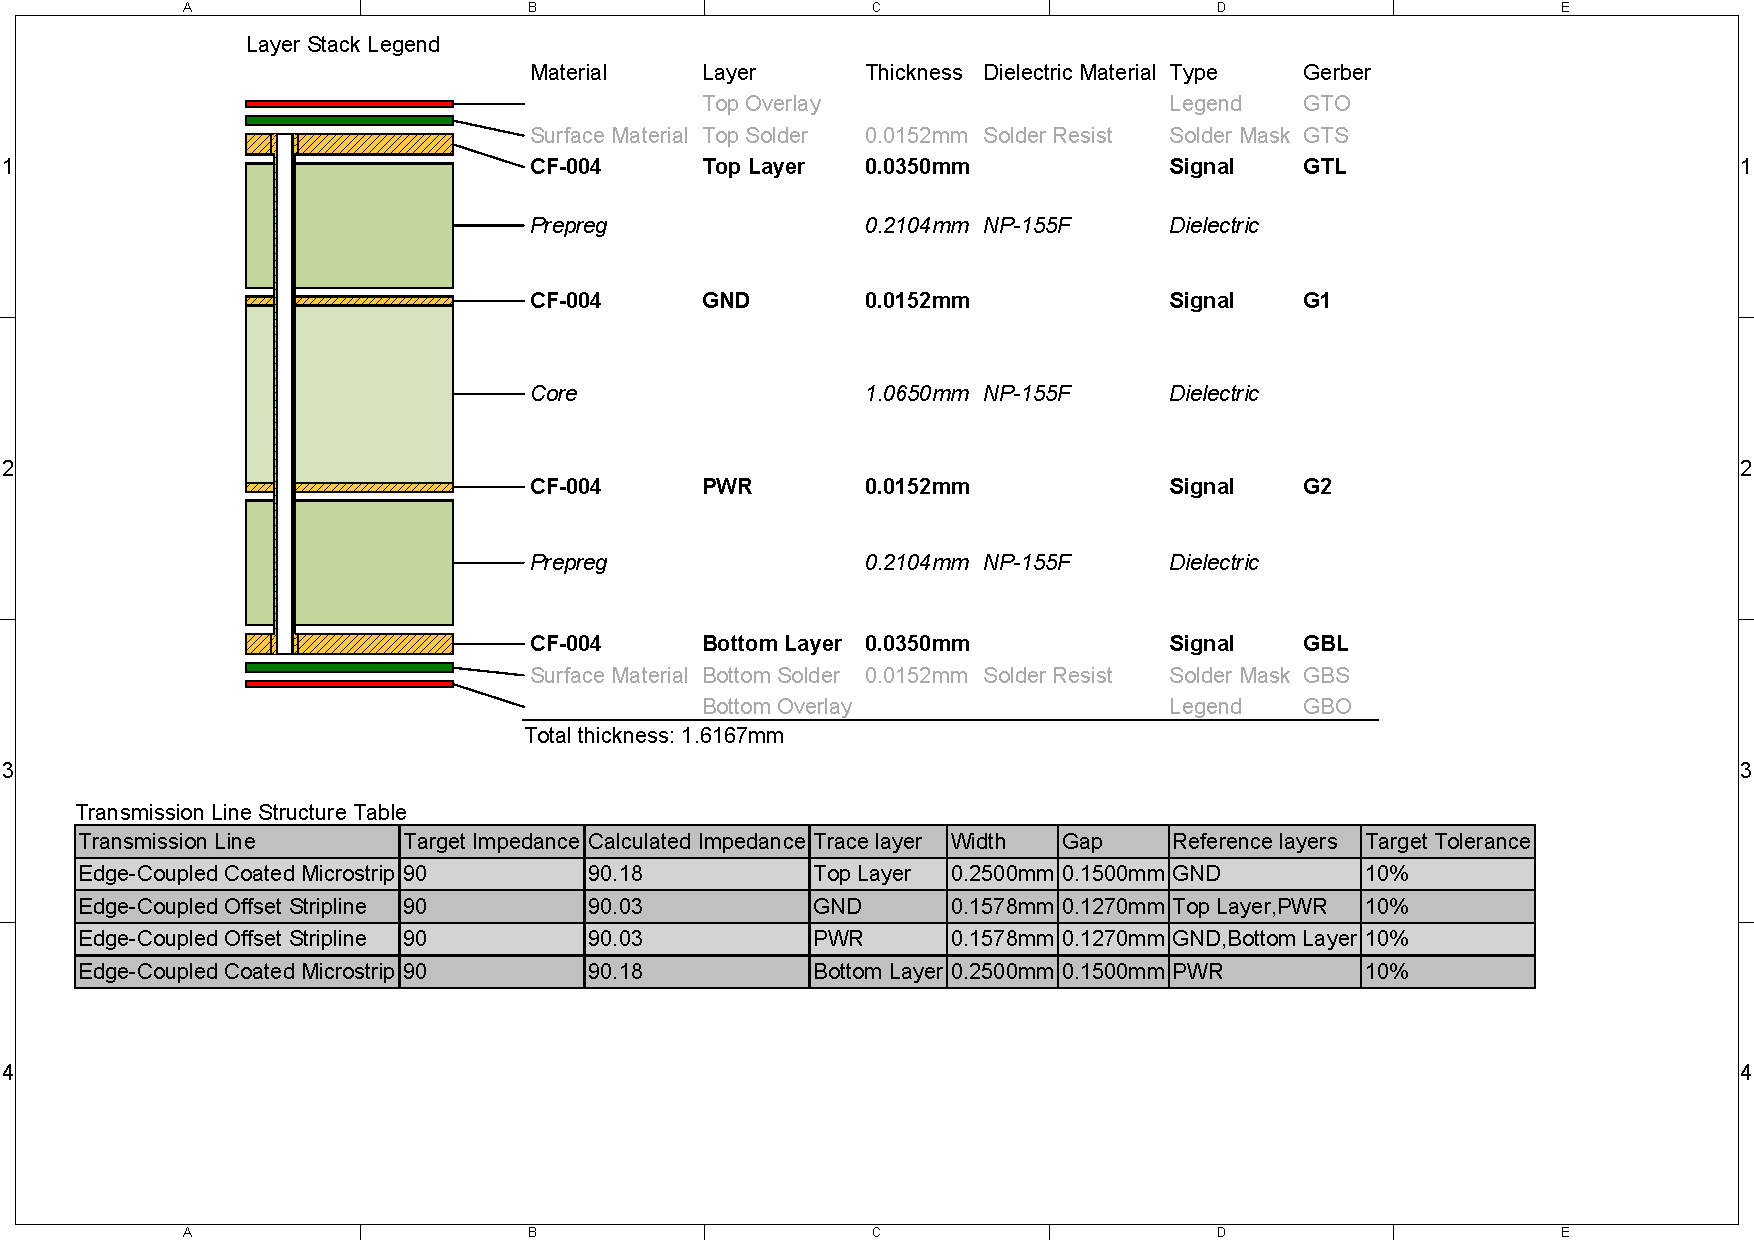
\includegraphics[width=0.8\textwidth, page=1, trim=34 119 103 14, clip]{BYTE_SPIne_Drawings.pdf}
\caption{Draftsman export: layer stack and differential impedance profile.}
\label{fig:stackup}
\end{figure}

% ---------------------------------------------------------------------------
\section{Test 2: Signal Integrity of the SPI1 Bus}\label{sec:si}

\subsection{Motivation and Topology}

The first version of the \maindoc{} assumed SPI edges of \qtyrange{5}{10}{ns} for all lines,
hence a critical length above \qty{130}{mm} and no need for any termination. SPI1 MOSI is the longest
line of the board (\qty{112}{mm}), close to that limit, so the assumption was checked with a simulation.
The simulation showed that it does not hold for the lines driven by the Jetson (Section~\ref{sec:limits});
the critical lengths of the main documentation have since been corrected (Table 11 there). The
topology of each SPI1 line is a \textbf{star at the pads of P2}: one branch on the top layer to MCU
B3, one branch (via to the bottom layer) to MCU B4.
\begin{itemize}[nosep]
    \item SCK, MOSI, NSS3, NSS4 are driven by the Jetson and received by the two MCUs;
    \item MISO is driven by the selected MCU through its \qty{33}{\ohm} series resistor R4 and received by
    the Jetson.
\end{itemize}
On the Jetson Orin Nano developer kit the 40-pin header is driven through \textbf{TXB0108} level
translators (\qty{1.8}{V} SoC side, port A; \qty{3.3}{V} header side, port B). The real driver of SCK/MOSI/NSS
is therefore the port B of a TXB0108, not the SoC.

\subsection{Acceptance Criteria}

A line passes when, at every receiver, the edge crosses the input threshold band \textbf{once} (monotonic
crossing) and the ringing after the edge does not re-enter the band:

\begin{table}[H]
\centering
\begin{tabular}{lccl}
\toprule
Receiver & $V_{IL}$ & $V_{IH}$ & Source \\
\midrule
STM32F072, FT pin, $V_{DD} = \qty{3.3}{V}$ & \qty{0.99}{V} & \qty{2.31}{V} & IBIS \texttt{io8p..\_sudq\_ft} \\
TXB0108 port B, $V_{CCB} = \qty{3.3}{V}$ & \qty{1.05}{V} & \qty{2.34}{V} & IBIS \texttt{TXB0108B\_IOB\_33} \\
\bottomrule
\end{tabular}
\caption{Input thresholds used as criteria (guaranteed values, 0.3/0.7\,$V_{DD}$).}
\label{tab:thresholds}
\end{table}

On a \textbf{clock} line a re-entry into the band can be seen as an extra edge (one bit too many). On
a \textbf{data} line it is harmless if the ringing has died out before the sampling edge of the clock (\qtyrange{125}{500}{ns}
after the data edge at \qtyrange{1}{4}{MHz}). The STM32 inputs have a Schmitt trigger;
the typical switching points (about \qtyrange{1.3}{1.6}{V}) are inside the band, which gives practical but
not guaranteed margin.

\subsection{IBIS Models}

\paragraph{STM32F072C8T6.} Downloaded from st.com~\cite{stibis} (product page, \textit{CAD Resources, IBIS models})
into \texttt{SI\_Models\textbackslash stm32f0\_ibis}. The archive contains one file per silicon family and package;
the number in the file name is the \textbf{DEV\_ID} of the family:

\begin{table}[H]
\centering
\begin{tabular}{ll}
\toprule
DEV\_ID & Family \\
\midrule
0x440 & STM32F030x8, STM32F05x \\
0x442 & STM32F09x, STM32F030xC \\
0x444 & STM32F03x (F030x4/x6, F031) \\
0x445 & STM32F04x, STM32F070x6 \\
\textbf{0x448} & \textbf{STM32F070xB, STM32F071, STM32F072} \\
\bottomrule
\end{tabular}
\caption{The file to use is \texttt{stm32f0\_448\_lqfp48.ibs}.}
\label{tab:devid}
\end{table}

\required{import \texttt{stm32f0\_448\_lqfp48.ibs}: \textbf{DEV\_ID 0x448} is the silicon of the
STM32F072. The other files of the archive belong to other STM32F0 families and give
wrong buffers.}

The file defines, for each pin type, a \textit{model selector} with several variants. For the FT pins
(PB12--PB15):

\begin{table}[H]
\centering
\begin{tabular}{l>{\raggedright\arraybackslash}p{0.6\textwidth}}
\toprule
Name part & Meaning (read from the file) \\
\midrule
\texttt{io8p01}, \texttt{io8p10}, \texttt{io8p11} & GPIO speed. Rise ramps $\approx\qty{12.5}{ns}$, \qty{6.4}{ns}, \qty{1.5}{ns}: \texttt{p01} is the slowest,
i.e.\ \textbf{Low speed} as configured in CubeMX \\
\texttt{\_lv} & supply \qty{2.0}{V} (thresholds 0.72/\qty{1.68}{V}) \\
no \texttt{\_lv} & supply \qty{3.3}{V} (thresholds 0.99/\qty{2.31}{V}) \\
\texttt{\_pd}, \texttt{\_pu} & internal pull-down / pull-up (\qty{40}{k\ohm}) enabled \\
\bottomrule
\end{tabular}
\caption{Model variants of the STM32 IBIS file.}
\label{tab:variants}
\end{table}

{\sloppy When importing, Altium converts each model into a \texttt{.mac} file and appends \texttt{\_tp} (typical
corner) and \texttt{\_in}/\texttt{\_out} (input/output part of the buffer): \texttt{io8p01\_sudq\_ft} becomes
\texttt{io8p01\_sudq\_ft\_tp\_in.mac} and \texttt{io8p01\_sudq\_ft\_tp\_out.mac}.\par}

\paragraph{TXB0108.} Downloaded from ti.com~\cite{tiibis} into \texttt{SI\_Models\textbackslash TXB0108\_IBIS\textbackslash txb0108.ibs} (component
\texttt{TXB0108YZP\_PW}). Port B is available at 1.8, 2.5, 3.3 and \qty{5}{V}, with and without the \textit{one-shot}
edge accelerator:

\begin{table}[H]
\centering
\begin{tabular}{lccc}
\toprule
Model & Behaviour & Edge ($\approx\qty{2}{V}$) & $C_\text{comp}$ \\
\midrule
\texttt{TXB0108B\_IOB\_33} & buffer without accelerator & \qty{0.6}{ns} & \qty{9.4}{pF} \\
\texttt{TXB0108\_IOB\_OS\_33} & one-shot active & \qtyrange{1.4}{2.5}{ns} & \qty{9.2}{pF} \\
\bottomrule
\end{tabular}
\caption{TXB0108 port B models at \qty{3.3}{V}.}
\label{tab:txbmodels}
\end{table}

The TXB0108~\cite{txbds} has a weak output (about \qty{4}{k\ohm}) and a one-shot that drives the line hard
for a few nanoseconds on every edge. TI states in the IBIS file that this change of impedance
during the transition cannot be described by IBIS and that the results may not be accurate. The
simulations of this document use \texttt{TXB0108B\_IOB\_33} (fastest edge), i.e.\ the \textbf{worst case}: a line
that passes with this model also passes with the real device.

\subsection{Procedure}

\subsubsection{Start and Model Assignments}

\begin{enumerate}
    \item \gui{Project \m Validate PCB Project}. From the PCB: \gui{Tools \m Signal Integrity}. The warning \textit{Not
    all components have Signal Integrity models set up} appears: \gui{Model Assignments\dots}.
    \item The table lists one entry per logical component (multi-channel: the model of U1 applies to
    the four MCUs). Passives (\textit{Low Confidence}) are modelled from their value and are correct.
    Components with \textit{No Match} that are not on the analysed nets (H1--H4, TP1--TP4, Y1, Y2,
    P3, D1, S1, S2) are ignored by the analyser and left as they are.
\end{enumerate}

\begin{dialog}
Errors or warnings found --- Not all components have Signal Integrity models set up.\\
\upshape\gui{[Model Assignments\dots] [Continue] [Cancel]}
\end{dialog}

\noindent This warning appears at every start, because some components on other nets have no model;
\gui{Continue} is correct once U1 and P2 are set.

\subsubsection{U1 (STM32)}

\begin{enumerate}
    \item Double-click on U1, Model Name \texttt{STM32F072C8\_LQFP48}, \textbf{Technology LVC} (see Section~\ref{sec:problems}),
    \gui{Import IBIS}, file \texttt{stm32f0\_448\_lqfp48.ibs}. The models are mapped to the pins
    by number (pin 44 BOOT0 receives \texttt{vpp\_test}, the I\textsuperscript{2}C pins the \texttt{i2c} models: the mapping
    is correct).
    \item The automatic choice is \texttt{io8p01\_sudq\_ft\_pd\_lv}: right speed, but \qty{2.0}{V} supply and internal
    pull-down, both wrong for this design. On the SPI2 pins set:
\end{enumerate}

\begin{table}[H]
\centering
\begin{tabular}{rlll}
\toprule
Pin & Signal & Input model & Output model \\
\midrule
25 & PB12, NSS  & \texttt{io8p11\_sudq\_ft\_tp\_in} & \texttt{io8p11\_sudq\_ft\_tp\_out} \\
26 & PB13, SCK  & \texttt{io8p11\_sudq\_ft\_tp\_in} & \texttt{io8p11\_sudq\_ft\_tp\_out} \\
27 & PB14, MISO & \texttt{io8p01\_sudq\_ft\_tp\_in} & \texttt{io8p01\_sudq\_ft\_tp\_out} (Low speed) \\
28 & PB15, MOSI & \texttt{io8p11\_sudq\_ft\_tp\_in} & \texttt{io8p11\_sudq\_ft\_tp\_out} \\
\bottomrule
\end{tabular}
\caption{U1 pin models. On the inputs only the input part is used, which is identical for all
speeds (same thresholds, $C_\text{comp} = \qty{1.97}{pF}$); the speed matters only on MISO, the only pin driven
by the MCU.}
\label{tab:u1models}
\end{table}

\required{set \textbf{Technology = LVC} in the component field of \textbf{U1 and P2} (not in the
per-pin column, which stays on \textit{Default}). With the default \textit{HC} every buffer is supplied at
\qty{5}{V} and all waveforms are wrong (Section~\ref{sec:problems}).}

\subsubsection{P2 (Jetson Header)}

\begin{enumerate}
    \item Double-click on P2, Type \textbf{IC}, Model Name \texttt{P2\_Jetson\_TXB0108}, \textbf{Technology LVC}, \gui{Import
    IBIS}, \texttt{txb0108.ibs}, component \texttt{TXB0108YZP\_PW}. The 20 pins of the TXB0108 are mapped
    by number onto pins 1--20 of P2, i.e.\ at random with respect to the board; only the analysed
    pins are corrected.
    \item \textbf{Problem:} the models cannot be edited, because all pins of P2 are \textit{Passive} (electrical type
    taken from the schematic). \textbf{Solution:} in the schematic select P2, \gui{Properties \m Pins}, pencil
    button (\textit{Component Pin Editor}), set \textit{Type} = \textbf{I/O} on pins 13, 16, 18, 22 and 37. P2 comes
    from Manufacturer Part Search, so this is a local change of the placed component; it does
    not affect the PCB nor the ERC.
    \item Validate the project, reopen Model Assignments and set on P2:
\end{enumerate}

\begin{table}[H]
\centering
\begin{tabular}{rlll}
\toprule
Pin & Signal & Input model & Output model \\
\midrule
13 & SPI1\_SCK  & \texttt{TXB0108B\_IOB\_33\_tp\_in} & \texttt{TXB0108B\_IOB\_33\_tp\_out} \\
37 & SPI1\_MOSI & \texttt{TXB0108B\_IOB\_33\_tp\_in} & \texttt{TXB0108B\_IOB\_33\_tp\_out} \\
18 & SPI\_NSS3  & \texttt{TXB0108B\_IOB\_33\_tp\_in} & \texttt{TXB0108B\_IOB\_33\_tp\_out} \\
16 & SPI\_NSS4  & \texttt{TXB0108B\_IOB\_33\_tp\_in} & \texttt{TXB0108B\_IOB\_33\_tp\_out} \\
22 & SPI1\_MISO & \texttt{TXB0108B\_IOB\_33\_tp\_in} & \texttt{TXB0108B\_IOB\_33\_tp\_out} \\
\bottomrule
\end{tabular}
\caption{P2 pin models (\qty{3.3}{V} port B). The automatic import had assigned the \qty{1.2}{V}/\qty{1.8}{V}
variants (first entries of the selectors); pins 13 and 16 had received the GND and OE models of
the TXB0108.}
\label{tab:p2models}
\end{table}

\required{the analysed pins of P2 (13, 16, 18, 22, 37) must have the electrical type \textbf{I/O} in
the schematic; with \textit{Passive} pins Altium does not let the models be edited.}

\subsubsection{Writing the Models to the Schematic}

At \gui{Analyze Design} Altium warns that \textit{some unsaved components have pin parameters} which are
not used unless written to the schematic. The per-pin models are such parameters: answer \gui{No},
tick \textit{Update Schematic} on the rows \textbf{U1} and \textbf{P2}, click \gui{Update Models in Schematic}, save, and
analyse again. The models become SI parameters of the two components; they have no effect on
PCB, DRC or BOM.

\required{after every change of the models, click \textbf{Update Models in Schematic} for U1
and P2 and save; otherwise the per-pin models are ignored by the analysis.}

\begin{dialog}
Some unsaved components have pin parameters. If these components have not been updated
on the schematic, any associated pin parameters will not be used during the analysis. Continue
Anyway?\quad\upshape\gui{[Yes] [No]}
\end{dialog}

\subsubsection{Analysis Setup and Rules}

The dialog \textit{SI Setup Options} applies only to nets that are not routed; all nets are routed, so the
real tracks and the stack-up of Section~\ref{sec:imp} are used and the defaults can be kept:

\begin{table}[H]
\centering
\begin{tabular}{lll}
\toprule
Setting & Value & Used for \\
\midrule
Track Impedance & \qty{100}{\ohm} & nets not yet transferred to the PCB \\
Average Track Length & \qty{2000}{mil} & nets placed but not routed \\
Use Manhattan length & enabled & nets placed but not routed \\
\bottomrule
\end{tabular}
\caption{SI Setup Options (defaults, not used for the routed SPI nets).}
\label{tab:setup}
\end{table}

The other settings are PCB rules (\gui{Design \m Rules \m Signal Integrity}). The table below is
generated from the rule export of the PCB (\gui{Design \m Rules}, right-click on \textit{Signal Integrity},
\gui{Export Rules}, file \texttt{SI\_Data\textbackslash BYTE\_SPIne.RUL}):

\begin{table}[H]
\centering
\small
\begin{tabular}{l>{\raggedright\arraybackslash}p{0.25\textwidth}>{\raggedright\arraybackslash}p{0.34\textwidth}}
\toprule
Rule (name in the export) & Value & Reason \\
\midrule
\texttt{SupplyNets\_5VUSB}       & \qty{5.000}{V} & \multirow{6}{=}{one rule per power net. Without them R3 (NSS pull-up) and the clamps of the
buffers have no reference: 3V3 and 5V were flagged red and the NSS nets were \textit{Not analyzed}} \\
\texttt{SupplyNets\_5V\_SPI}     & \qty{5.000}{V} & \\
\texttt{SupplyNets\_5V}          & \qty{5.000}{V} & \\
\texttt{SupplyNets\_3V3\_Jetson} & \qty{3.300}{V} & \\
\texttt{SupplyNets\_3V3}         & \qty{3.300}{V} & \\
\texttt{SupplyNets\_GND}         & \qty{0.000}{V} & \\
\midrule
\texttt{SignalStimulus} & single pulse, low start, \qtyrange{10}{60}{ns}, period \qty{100}{ns} & default; only the edges matter for reflections \\
\texttt{SignalTopValue} & min.\ \qty{3.300}{V} & pass criterion for the high level (default \qty{5}{V}) \\
Signal Base Value & \textbf{deleted} & with a maximum of \qty{0}{V} every net fails on a few microvolts; without the rule the base
level is not checked, which is acceptable because the waveforms are judged directly \\
\bottomrule
\end{tabular}
\caption{Signal integrity rules (from \texttt{BYTE\_SPIne.RUL}). The export also contains the rule
\textit{Schematic Supply Nets} (GND, \qty{0}{V}), created automatically by Altium from the power ports
of the schematic. The scope of each Supply Nets rule is \texttt{InNet('<net>')}, the scope of the other
rules is \textit{All}.}
\label{tab:rules}
\end{table}

\required{define \textbf{one Supply Nets rule per power net} and \textbf{delete the Signal Base
Value rule}; without the first the pull-ups and clamps have no reference, with the second
almost every net fails on a meaningless criterion.}

\subsubsection{Running a Reflection Analysis}

\begin{enumerate}
    \item In the Signal Integrity panel, double-click on the net (or select it and click \gui{>}): it moves to
    the list on the right and its pins are listed below.
    \item Right-click on each pin and set the direction: the driver \textbf{Out}, the receivers \textbf{In} (Table~\ref{tab:directions}).
    \item \gui{Reflection Waveforms\dots}. The result opens as a separate document \texttt{BYTE\_SPIne.sdf}, one
    tab per run.
    \item For a termination sweep tick \textbf{Serial Res} in the Termination list (\textit{No Termination} cannot
    be unticked: it is always simulated as reference), keep \textit{Perform Sweep} with 10 steps; the
    series resistor is placed at the driver.
\end{enumerate}

\begin{table}[H]
\centering\small
\begin{tabular}{lll}
\toprule
Net & Out & In \\
\midrule
SPI1\_MOSI & P2-37 & U1\_CAN\_B3-28, U1\_CAN\_B4-28 \\
SPI1\_SCK  & P2-13 & U1\_CAN\_B3-26, U1\_CAN\_B4-26 \\
SPI1\_MISO & U1\_CAN\_B4-27 (farthest MCU) & P2-22, U1\_CAN\_B3-27 (high impedance) \\
\bottomrule
\end{tabular}
\caption{Pin directions.}
\label{tab:directions}
\end{table}

\required{set the directions of every analysed net before each run: the driver \textbf{Out}, the
receivers \textbf{In}. With inverted directions the waveforms describe a different circuit (Section~\ref{sec:problems}).}

\subsection{Problems Found and Solutions}\label{sec:problems}

\begin{table}[H]
\centering
\begin{tabular}{>{\raggedright\arraybackslash}p{0.3\textwidth}>{\raggedright\arraybackslash}p{0.3\textwidth}>{\raggedright\arraybackslash}p{0.3\textwidth}}
\toprule
Symptom & Cause & Solution \\
\midrule
P2 models cannot be edited & P2 pins are Passive in the schematic & electrical type I/O on the SPI1 pins (Component Pin Editor) \\
Warning about pin parameters & per-pin models are used only if written to the schematic & \gui{Update Models in Schematic} for U1 and P2 \\
3V3/5V red, NSS nets \textit{Not analyzed} & no Supply Nets rule & one Supply Nets rule per power net \\
\gui{Reflection Waveforms} does nothing & no net in the list on the right & move the net with \gui{>} or double-click \\
All waveforms swing \qty{0}{V} to \qty{5}{V}, Top Value \qty{5.000}{V} on every net & component Technology \textit{HC} (74HC family, \qty{5}{V}) & Technology \textbf{LVC} on U1 and P2 (Section~\ref{sec:problems}) \\
Almost every net fails after changing the rules & Base Value maximum \qty{0}{V}; overshoot measured against the Top Value (\qty{3.3}{V}), so nets still at \qty{5}{V} show $\approx\qty{1.7}{V}$ of ``overshoot'' & Signal Base Value rule deleted; judge the result on the waveforms, not on the screening table \\
MISO waveform unrealistic & directions inverted (P2 set as driver) & U1\_CAN\_B4-27 Out, P2-22 In \\
Screening and waveforms disagree (e.g.\ MOSI overshoot \qty{2.53}{V} in the table, $\approx\qty{0.7}{V}$ on the waveform) & the screening is a fast approximate calculation & use the screening only to choose the nets to simulate \\
\bottomrule
\end{tabular}
\caption{Problems met during the setup.}
\label{tab:problems}
\end{table}

\paragraph{Screening of the final layout.} The screening table of the Signal Integrity panel is exported
with a right-click on the net list, \gui{Display Report}; Altium writes \texttt{Signal Integrity Tests
Report.txt} in the project folder (copy in \texttt{SI\_Data\textbackslash si\_screening\_report.txt}). The report
lists, for each criterion, only the nets outside the tolerance (\qty{0.66}{V} for the SPI1 nets). The SPI1
rows:

\begin{table}[H]
\centering
\small
\setlength{\tabcolsep}{4pt}
\begin{tabular}{>{\raggedright\arraybackslash}p{0.25\textwidth}ccccc}
\toprule
Net & \shortstack{Falling edge\\overshoot} & \shortstack{Falling edge\\undershoot} & \shortstack{Rising edge\\overshoot} & \shortstack{Rising edge\\undershoot} & Top Value \\
\midrule
SPI1\_MOSI & \qty{2.513}{V} & \qty{1.637}{V} & \qty{2.361}{V} & \qty{1.484}{V} & pass \\
SPI1\_SCK (MCU side) & \qty{1.407}{V} & pass & \qty{1.240}{V} & pass & pass \\
NetP2\_13 (P2 side) & \qty{1.407}{V} & pass & \qty{1.240}{V} & pass & pass \\
SPI1\_MISO,\newline NetR4\_CAN\_B3/B4\_1 & pass & pass & pass & pass & \qty{3.292}{V} \\
\bottomrule
\end{tabular}
\caption{Screening of the SPI1 nets on the final layout (\texttt{si\_screening\_report.txt}). ``pass''
means that the net is not listed for that criterion. SPI1\_SCK and NetP2\_13 are the two sides
of R17.}
\label{tab:screening}
\end{table}

The Top Value of the SPI1 nets is \qty{3.3}{V} (MISO \qty{3.292}{V}, below the minimum of \qty{3.3}{V} only
because of the drop on R4), which confirms that the \qty{3.3}{V} configuration of Section~\ref{sec:problems} is active.
The overshoot values, instead, do not match the waveforms (for example \qty{2.5}{V} for MOSI) and
do not change with R17 on SCK: the screening is a fast approximate calculation, used here only
to choose the nets to simulate.

\paragraph{The \qty{5}{V} swing.} The first waveforms swung from 0 to \qty{5}{V} on driver and receivers, although
all models are \qty{3.3}{V} models: on SPI1\_MOSI the driver P2-37 settled at \qty{5.0}{V} and the receivers
peaked at about \qty{5.5}{V} (B3) and \qty{5.7}{V} (B4). The shape of the ringing was correct, only the
amplitude was wrong. Two attempts had no effect: setting the Supply Nets rule of 5V\_SPI
(the \qty{5}{V} pins of P2) to \qty{3.3}{V}, and setting the Signal Top Value rule to \qty{3.3}{V} (it is only a pass
criterion). The cause is the field \textbf{Technology} of the component in the model dialog, which
defaults to \textit{HC} (74HC logic, \qty{5}{V}) and sets the supply of the buffers. Setting it to \textbf{LVC} (\qty{3.3}{V}
CMOS) on U1 and P2, writing the models to the schematic and re-analysing gives the correct
\qty{3.3}{V} swing. Only the component field must be changed: the per-pin Technology column stays
on \textit{Default}, otherwise the generic LVC models could replace the IBIS models.

\required{when reproducing the analysis, check the column \textbf{Top Value} of the SPI1 nets
($\approx\qty{3.3}{V}$) \textbf{before reading any waveform}.}

The 5V\_SPI rule was set back to \qty{5}{V}. The Technology list of the model dialog offers the
logic families of the generic models (GTL\_LVT, HC, HCT, HLL, LS, LV, LVC, \dots); LVC is the
\qty{3.3}{V} CMOS family.

\paragraph{Inverted MISO directions.} In a first MISO run P2 was set as driver by mistake. With the
fast TXB0108 edge driving the branched line, the MCU pins showed a ringing up to about \qty{4.3}{V}
(B3) and \qty{4.7}{V} (B4) and an undershoot of about $-\qty{0.8}{V}$. This is not the real case (MISO is
driven by the MCU through R4), but it shows the same effect that is found later on SCK and
MOSI.

\subsection{Results}\label{sec:results}

The waveforms were exported from the SimData document (click in a plot, \gui{File \m Export \m Plot},
CSV) and plotted with \texttt{plot\_si.py} (Section~\ref{sec:changes}); all values below are computed from the exported
data. The threshold band of each receiver is shaded. Definitions:
\begin{itemize}[nosep]
    \item \textit{minimum after rise}: lowest point of the ringing after the first overshoot peak (a shoulder
    on the edge itself, above $V_{IH}$, is not a re-entry);
    \item \textit{maximum after fall}: highest point of the ringing after the first undershoot;
    \item \textit{margin}: minimum after rise $-V_{IH}$, and $V_{IL}-$ maximum after fall.
\end{itemize}

\begin{table}[H]
\centering
\small\setlength{\tabcolsep}{4pt}
\begin{tabular}{llrrrrcl}
\toprule
Net & Receiver & Peak & \shortstack[r]{Min.\ after\\rise} & \shortstack[r]{Max.\ after\\fall} & \shortstack[r]{Under-\\shoot} & \shortstack{Margin\\high / low} & Verdict \\
\midrule
MISO & P2-22 (Jetson) & 4.51 & 2.77 & 0.28 & $-0.75$ & $+0.43$ / $+0.77$ & pass \\
MISO & B3-27 & 4.60 & 2.72 & 0.32 & $-0.78$ & $+0.41$ / $+0.67$ & pass \\
\midrule
MOSI & B3-28 & 5.04 & 1.85 & 0.62 & $-0.80$ & $-0.46$ / $+0.37$ & acceptable (data) \\
MOSI & B4-28 & 5.31 & 1.60 & 0.63 & $-0.80$ & $-0.71$ / $+0.36$ & acceptable (data) \\
\midrule
SCK, no R & B3-26 & 4.79 & 2.18 & 0.55 & $-0.79$ & $-0.13$ / $+0.44$ & marginal \\
SCK, no R & B4-26 & 4.91 & 2.09 & 0.53 & $-0.78$ & $-0.22$ / $+0.46$ & marginal \\
\textbf{SCK}, \qty{33}{\ohm} & B3-26 & 3.71 & 2.96 & 0.28 & $-0.29$ & $+0.65$ / $+0.71$ & \textbf{pass} \\
\textbf{SCK}, \qty{33}{\ohm} & B4-26 & 4.10 & 2.79 & 0.42 & $-0.76$ & $+0.48$ / $+0.57$ & \textbf{pass} \\
\bottomrule
\end{tabular}
\caption{Results in volts (worst-case driver model). Thresholds: STM32 0.99/\qty{2.31}{V}, TXB0108
1.05/\qty{2.34}{V}. ``SCK, \qty{33}{\ohm}'' is the analysis of the final layout, with the resistor placed and routed.}
\label{tab:results}
\end{table}

\paragraph{MISO.} The driver waveform at B4 is clean and shows the typical step of a source-terminated
line: R4 (\qty{33}{\ohm}) works as intended. The remaining ringing at the Jetson comes from the star
topology, where the branch to B3 acts as an unterminated stub; it stays out of the threshold
band with \qty{0.43}{V} of margin. The overshoot (\qty{4.5}{V}) is within the absolute maximum of the
TXB0108 inputs (\qty{6.5}{V}); the undershoot of $-\qty{0.75}{V}$ for about \qty{2}{ns} slightly exceeds the $-\qty{0.5}{V}$
rating, with the current limited by R4, and will be reduced on the real board by the capacitance
of the Jetson carrier, which is not modelled.

\begin{figure}[H]
\centering
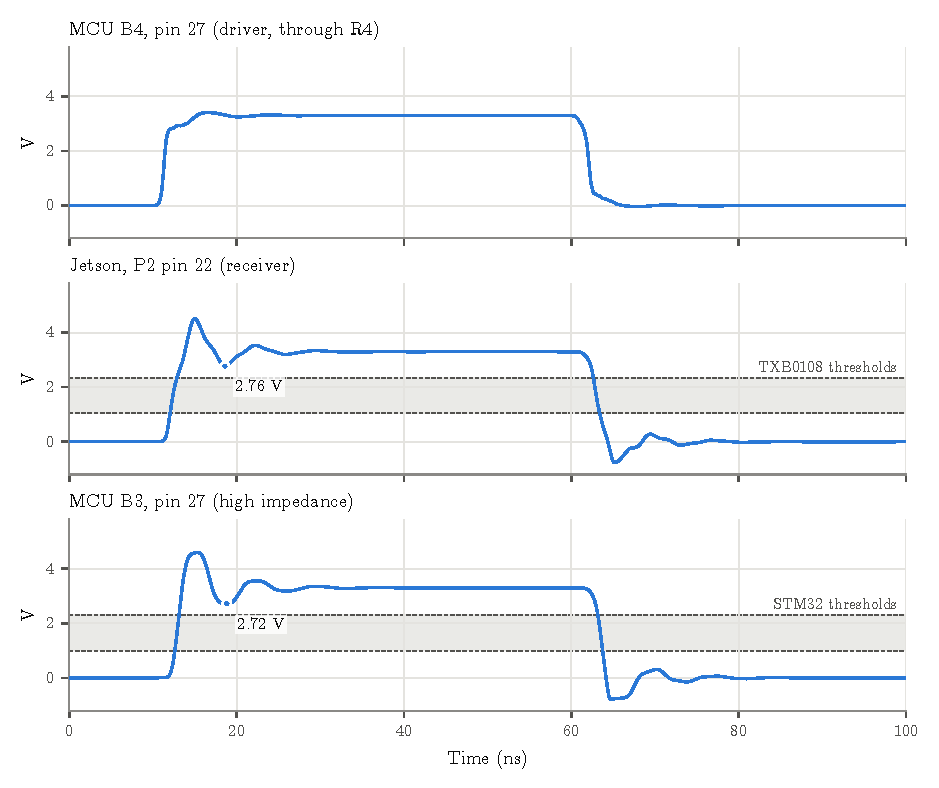
\includegraphics[width=\textwidth]{SI_Figures/si_wave_miso.pdf}
\caption{SPI1\_MISO, MCU B4 driving through R4.}
\label{fig:miso}
\end{figure}

\paragraph{MOSI.} The ringing after the rising edge re-enters the threshold band at both MCUs, by up to
\qty{0.71}{V} at B4. MOSI is a data line sampled on the clock edge, \qtyrange{125}{500}{ns} after the data edge
at \qtyrange{1}{4}{MHz}, while the ringing has left the band about \qty{20}{ns} after the edge: the value is
stable when it is sampled. Acceptable without termination.

\begin{figure}[H]
\centering
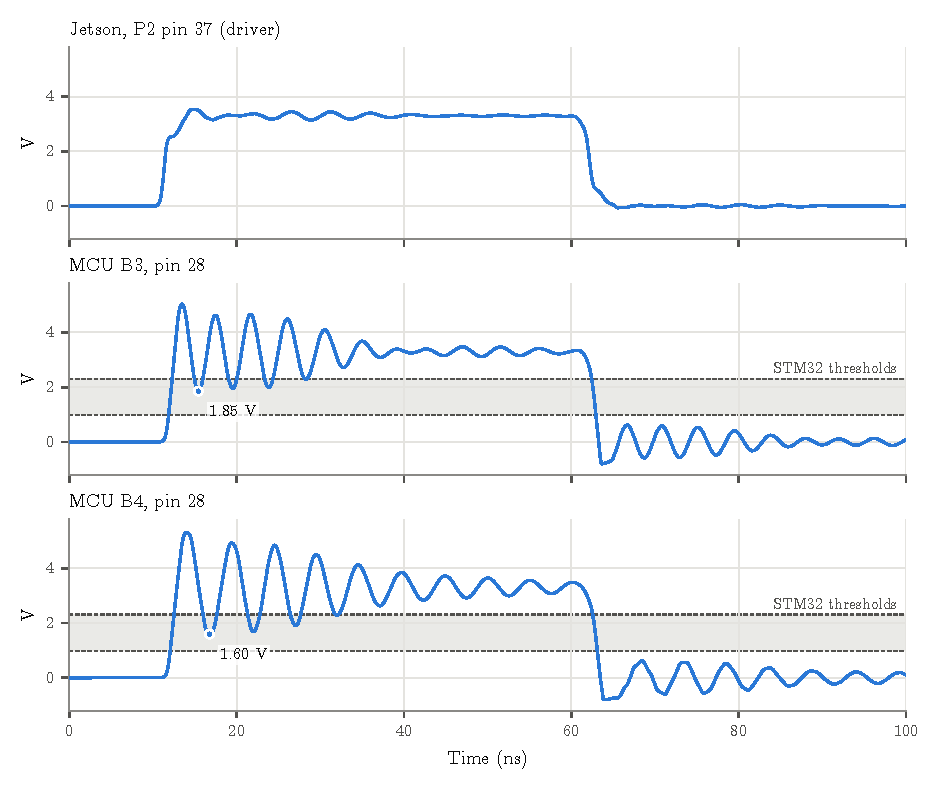
\includegraphics[width=\textwidth]{SI_Figures/si_wave_mosi.pdf}
\caption{SPI1\_MOSI, Jetson driving.}
\label{fig:mosi}
\end{figure}

\paragraph{SCK.} Without series resistor the first ring after the rising edge falls to \qty{2.09}{V} at B4 and \qty{2.18}{V}
at B3, i.e.\ \qtyrange{0.13}{0.22}{V} below the guaranteed $V_{IH}$, and the line keeps ringing during the
whole pulse (resonance of the star). It stays far above $V_{IL}$ and above the typical switching point
of the Schmitt trigger, so a double clock is unlikely, but the margin with respect to the datasheet
is negative on the line where an extra edge costs a bit. With the \qty{33}{\ohm} resistor placed and routed
on the layout (Figure~\ref{fig:sck}, blue) the first ring stays at \qty{2.79}{V} (B4) and \qty{2.96}{V} (B3): margin \qty{0.48}{V}
or more, peak reduced from 4.9 to \qty{4.1}{V}. The driver waveform at P2 is practically unchanged.

\begin{figure}[H]
\centering
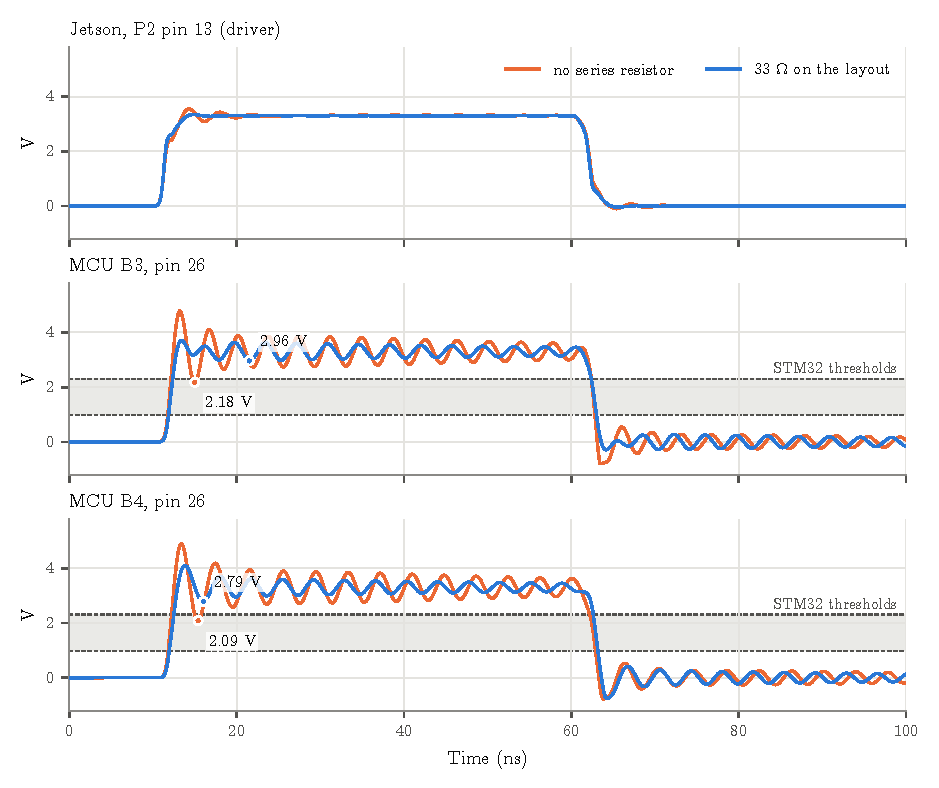
\includegraphics[width=\textwidth]{SI_Figures/si_wave_sck.pdf}
\caption{SPI1\_SCK before (orange) and after (blue) the \qty{33}{\ohm} series resistor, analysis of the
final layout. The marked points are the minima after the rising edge.}
\label{fig:sck}
\end{figure}

\paragraph{Series-resistor sweep.} Before the layout change, the sweep of the Signal Integrity panel
(\textit{Serial Res}, 10 to \qty{56}{\ohm} in 10 linear steps of \qty{5.1}{\ohm}, resistor ideally placed at the driver) was used
to choose the value. The minimum after rise at B4 grows monotonically from \qty{2.54}{V} (\qty{10}{\ohm})
to \qty{3.12}{V} (\qty{56}{\ohm}), and the peak falls from 4.52 to \qty{3.53}{V}: every value of the range removes the
re-entry. Larger values also slow down the edge, so a value in the middle of the range is the right
compromise. The layout result with \qty{33}{\ohm} (\qty{2.79}{V}) is about \qty{0.15}{V} lower than the sweep at the
same value (\qtyrange{2.95}{3.00}{V}), because on the board the resistor sits a few millimetres from the
pad and the bottom branch starts after a via; the margin is still ample.

\begin{figure}[H]
\centering
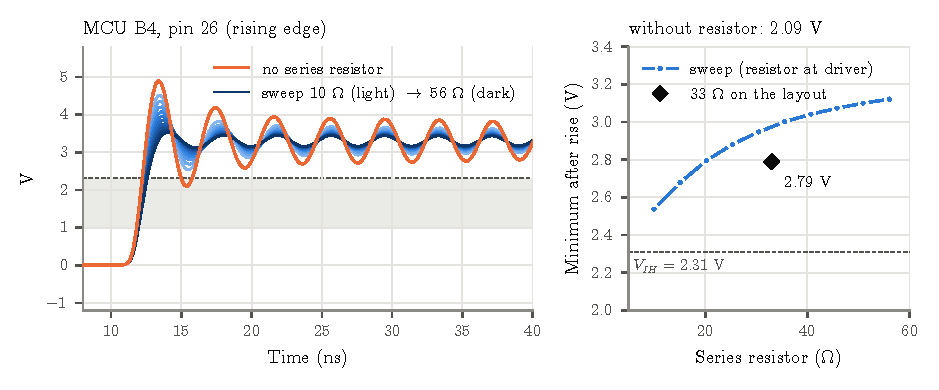
\includegraphics[width=\textwidth]{SI_Figures/si_wave_sck_sweep.pdf}
\caption{SPI1\_SCK at MCU B4: rising edge for the ten values of the sweep (left) and minimum
after rise as a function of the series resistor (right), with the result of the final layout.}
\label{fig:sweep}
\end{figure}

\subsection{Interpretation and Limits}\label{sec:limits}

\begin{itemize}
    \item \textbf{The assumption of the first version of the main documentation is not valid for
    the Jetson-driven lines.} The STM32 at low speed has edges of $\approx\qty{12}{ns}$ (MISO is clean),
    but the TXB0108 drives edges of \qtyrange{0.6}{2.5}{ns}. With \qty{6.5}{ps/mm} and the one-sixth rule,
    the critical length becomes
    \[
    l_\text{crit} = \frac{t_r}{6 \cdot \qty{6.5}{ps/mm}} \approx \qty{15}{mm}\ (t_r = \qty{0.6}{ns})\ \dots\ \qty{64}{mm}\ (t_r = \qty{2.5}{ns}),
    \]
    so the \qty{112}{mm} lines in star topology are transmission lines.
    \item \textbf{Worst case.} The driver model without one-shot has the fastest edge; the real TXB0108
    returns to its \qty{4}{k\ohm} output after the one-shot, which damps the ringing.
    \item \textbf{Not modelled:} the track of the Jetson carrier between the TXB0108 and the header, the
    header itself and any losses of the dielectric (the simulation is lossless). All of them reduce
    the ringing. The \textbf{40-way ribbon cable} between the Jetson and the board is not modelled
    either and can change the result substantially: SCK must therefore be measured on the
    prototype with the final cable (Section~\ref{sec:open}).
    \item \textbf{IBIS accuracy:} TI states that IBIS cannot describe the dynamic impedance of the
    TXB0108; the results are an order of magnitude, not a measurement.
    \item \textbf{SPI0} was not simulated (its pins on P2 are still Passive). Its topology is the same star at
    P2, so the conclusions are applied to SPI0 by similarity.
\end{itemize}

\subsection{Design Decision}\label{sec:decision}

One \qty{33}{\ohm} \textbf{series resistor} has been added on each SCK line (SPI0\_SCK at P2 pin 23, SPI1\_SCK
at P2 pin 13), on the top layer, within \qtyrange[range-phrase=--, range-units=single]{3}{5}{mm} of the pad of P2 and \textbf{before} the branch point:

\begin{center}
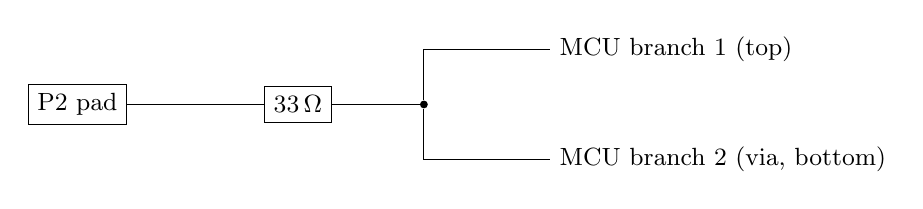
\begin{tikzpicture}[font=\small]
    \node[draw] (p2) at (0,0) {P2 pad};
    \node[draw] (r) at (2.8,0) {\qty{33}{\ohm}};
    \draw (p2) -- (r);
    \draw (r.east) -- (4.4,0) node[circle, fill, inner sep=1pt] (b) {};
    \draw (b) |- (6.0,0.7) node[right] {MCU branch 1 (top)};
    \draw (b) |- (6.0,-0.7) node[right] {MCU branch 2 (via, bottom)};
\end{tikzpicture}
\end{center}

\begin{itemize}[nosep]
    \item a source termination works only close to the driver; P2 is the closest point available on the
    board, and it is where Altium placed the resistor in the sweep;
    \item on the layout the branch point is a via next to the resistor: the top branch leaves the
    resistor pad, the bottom branch leaves the via (a via connects both layers at the same
    point);
    \item \qty{33}{\ohm} is the same part as R4: no new BOM line and no extra JLCPCB setup fee (Basic
    part);
    \item $\qty{33}{\ohm} \times \qty{40}{pF} \approx \qty{1.3}{ns}$: negligible at \qtyrange{1}{4}{MHz};
    \item damping the reflection that returns to the TXB0108 also protects its one-shot from being
    re-triggered, a known issue of this translator on long lines;
    \item MOSI (data, sampled after the ringing) and NSS (stays below $V_{IL}$ after the falling edge,
    to be confirmed) do not need a resistor; one per MOSI line can be added if space allows.
\end{itemize}

% ---------------------------------------------------------------------------
\section{Changes Made to the Project for the Simulations}\label{sec:changes}

\begin{table}[H]
\centering
\begin{tabular}{>{\raggedright\arraybackslash}p{0.36\textwidth}>{\raggedright\arraybackslash}p{0.56\textwidth}}
\toprule
Where & Change \\
\midrule
Schematic, P2 & electrical type of pins 13, 16, 18, 22, 37 changed from Passive to I/O (local change of the placed part; an
\textit{Update From Library} restores Passive) \\
Schematic, U1 and P2 & SI model parameters (IBIS models per pin) written with \gui{Update Models in Schematic} \\
PCB rules & Supply Nets (6 rules), Signal Top Value \qty{3.3}{V}, Signal Base Value rule deleted; 5V\_SPI temporarily set to \qty{3.3}{V}
and restored to \qty{5}{V} \\
Schematic, U1 and P2 (SI models) & Technology LVC instead of HC \\
Schematic and PCB & two \qty{33}{\ohm} series resistors on SPI0\_SCK and SPI1\_SCK (design change resulting from the simulation) \\
Documentation & CSV exports of the waveforms in \texttt{Documentation\textbackslash SI\_Data}, plotting script \texttt{plot\_si.py} \\
Layer Stack Manager & impedance profiles S50 and D90 (USB 90R) \\
Project & new Draftsman document \texttt{BYTE\_SPIne.PCBDwf}; folder \texttt{SI\_Models} with the IBIS files \\
\bottomrule
\end{tabular}
\caption{Changes. Apart from the two resistors, none of them affects copper, DRC or BOM;
the SI rules are not checked by the DRC unless enabled.}
\label{tab:changes}
\end{table}

\section{Open Points}\label{sec:open}

\paragraph{Status of the prototype (26 November 2026).} The BYTE SPIne has been tested and validated
in USB mode and works without errors, which is consistent with the USB impedance result of
Section~\ref{sec:imp}. The SPI mode has not been tested yet: the SPI1 results of Section~\ref{sec:si} are
therefore not yet confirmed by a measurement, and point 5 below is still open.

\begin{enumerate}
    \item Repeat SCK with the realistic driver model \texttt{TXB0108\_IOB\_OS\_33\_tp\_out} on P2-13.
    \item Reflection analysis of NSS3/NSS4, in particular the falling edge (slave selection).
    \item Crosstalk SCK $\to$ NSS: select both nets, right-click on SCK, \gui{Set Aggressor}, \gui{Crosstalk Waveforms};
    compare with the estimate of \qtyrange{10}{15}{mV} of the \maindoc{} (Section 9.5).
    \item Repeat the SCK analysis of SPI0 on the layout with its resistor (pins of P2 set to I/O as
    for SPI1).
    \item Bench test on the prototype: SCK at both MCUs with an oscilloscope (probe with short
    ground spring), with the final ribbon cable, and the SPI test of 10\,min listed in the \maindoc{} (Section 11).
\end{enumerate}

\section{Quick Reproduction Checklist}

\begin{enumerate}[nosep]
    \item Stack-up as Figure~\ref{fig:stackup}, impedance profile D90 (Section~\ref{sec:imp}).
    \item IBIS files in \texttt{SI\_Models}: \texttt{stm32f0\_448\_lqfp48.ibs}, \texttt{txb0108.ibs}.
    \item P2 pins 13, 16, 18, 22, 37 electrical type I/O.
    \item \gui{Tools \m Signal Integrity \m Model Assignments}: U1 and P2 as in the tables above, \gui{Update
    Models in Schematic}.
    \item Technology LVC on U1 and P2. Rules: Supply Nets, Signal Top Value \qty{3.3}{V}, no Signal
    Base Value rule.
    \item \gui{Reanalyze Design}; check Top Value $\approx\qty{3.3}{V}$ on the SPI1 nets.
    \item Net to the right list, directions as Table~\ref{tab:directions}, \gui{Reflection Waveforms}; Serial Res (\qtyrange[range-phrase=--, range-units=single]{10}{56}{\ohm}, 10
    steps) for the sweep.
    \item Export: click in a plot, \gui{File \m Export \m Plot}, CSV; figures with \texttt{python plot\_si.py
    SI\_Data SI\_Figures}.
\end{enumerate}

\addcontentsline{toc}{section}{References}
\begin{thebibliography}{9}
\bibitem{main} J. Luca, \textit{Architecture Design and Sizing of the BYTE SPIne SPI-to-CAN Bridge}, BARK
Project, October 2026, \href{run:BYTE_SPIne_Documentation.pdf}{\texttt{Documentation/BYTE\_SPIne\_Documentation.pdf}}.
\bibitem{stibis} STMicroelectronics, \textit{STM32F0 IBIS models}, file \texttt{stm32f0\_448\_lqfp48.ibs}, rev.~1.0, product
page (\textit{CAD Resources}): \url{https://www.st.com/en/microcontrollers-microprocessors/stm32f072c8.html}.
\bibitem{tiibis} Texas Instruments, \textit{TXB0108 IBIS model}, file \texttt{txb0108.ibs}, rev.~1.7, product page (\textit{Design
\& development}): \url{https://www.ti.com/product/TXB0108}.
\bibitem{txbds} Texas Instruments, \textit{TXB0108 8-Bit Bidirectional Voltage-Level Translator with Auto-Direction
Sensing}, datasheet, \url{https://www.ti.com/product/TXB0108}.
\bibitem{ipc2141} IPC, \textit{IPC-2141A Design Guide for High-Speed Controlled Impedance Circuit Boards}; paid
standard, \url{https://www.ipc.org}.
\bibitem{altiumsi} Altium, \textit{Signal Integrity Analysis (by Altium)}, \url{https://www.altium.com/documentation/altium-designer/analyzing-pcb/si-analysis/si-analyzer-altium}.
\bibitem{altiumstack} Altium, \textit{Defining the Layer Stack}, \url{https://www.altium.com/documentation/altium-designer/pcb/defining-layer-stack}.
\bibitem{altiumtlt} Altium, \textit{Draftsman Transmission Line Table}, \url{https://altium.com/documentation/altium-nexus/draftsman-transmission-line-table}.
\bibitem{jlcimp} JLCPCB, \textit{Impedance calculator}, \url{https://jlcpcb.com/capabilities/impedance-calculator}.
\end{thebibliography}

\end{document}
